\documentclass[french,12pt,notitlepage]{report}
\usepackage[utf8]{inputenc}
\usepackage[T1]{fontenc}
\usepackage{lmodern}
\usepackage[a4paper]{geometry}
\usepackage[francais]{babel}
\usepackage{graphicx}
\usepackage{amssymb}
\usepackage{amsmath}


\begin{document}
	\title{Functional data analysis applied to neurology}
	\author{Clément Bonvoisin, Pierre Ludmann}
	\date{30 juin 2014}
	\maketitle

	\begin{abstract}
  
Il s'agit de segmenter des signaux de marche,
dans le cadre d'une collaboration du CMLA (ENS Cachan) et Cognac-G (Paris V).
%Quels sont les travaux déjà accomplis dans ce domaine dans le monde?

On propose donc ici des algorithmes pour détecter des ruptures.
Cela permet en aval aux médecins de mieux étudier les différents régimes de marche.
Un algorithme efficace et rapide semble encore manquer.

Si la détection d'un unique changement trouve des implémentations reconnues,
on a cherché à généraliser à de multiples ruptures.
Aussi on a changé le paramètre de décision : on exige un nombre précis de résultats plutôt qu'un seuil de détection.

Malgré de fortes hypothèses de travail,
on obtient des résultats statisfaisants sur des signaux réels et synthétiques
bien que des améliorations restes possibles.

Son utilisation doit faire place à un apprentissage sur les segments de régime obtenus.
	
	\end{abstract}

	\tableofcontents

	\chapter{Introduction au problème}
	\section{Motivations}
		La motivation initiale de ce stage provient de la médecine, et plus particulièrement de la neurologie. Le projet, piloté par le groupe Cognac-G, vise à analyser en détail des signaux physiologiques, issus d'une expérience très simple.
	\\ \\
	Le protocole expérimental se décline comme suit :
	\begin{itemize}
		\item On place sur le patient un ensemble de capteurs : un à la tête, un à la ceinture, et un sur chaque pied. Ces capteurs sont des centrales inertielles, qui permettent une mesure de l'accélération et de la vitesse angulaire du patient.
		\item On lance l'acquisition. Pendant quelques secondes, le patient est à l'arrêt. Puis, il commence à marcher sur une dizaine de mètres, effectue un demi-tour, et fait une marche retour. Il s'arrête, et on peut alors arrêter l'acquisition.
		\item On replace alors les signaux obtenus dans un repère adapté au corps humain, formé de trois axes : l'axe antéro-postérieur, l'axe transversal (aussi appelé médio-latéral), et l'axe longitudinal (aussi appelé axe vertical).
	\end{itemize}
	
	\begin{figure}[!h]
		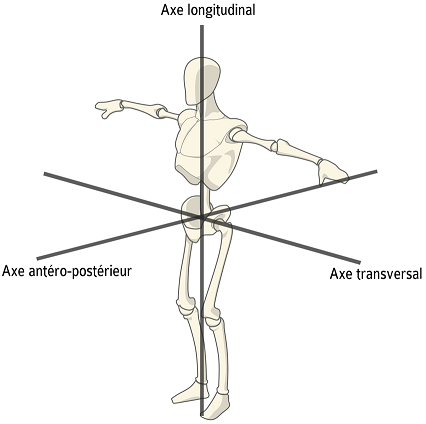
\includegraphics[scale=0.3]{axis.png}
		\caption{Le repère (antéro-postérieur; médio-latéral; vertical)}
		\label{axis}
	\end{figure}
		
	\vspace{1pc}
	
	On obtient alors des signaux physiologiques ayant 6 composantes distinctes pour chaque capteur, à une fréquence d'acquisition dépendante de la centrale inertielle utilisée ; actuellement, le projet Cognac-G dispose d'instruments permettant un échantillonnage à 100Hz.
	
	\begin{figure}[!h]
		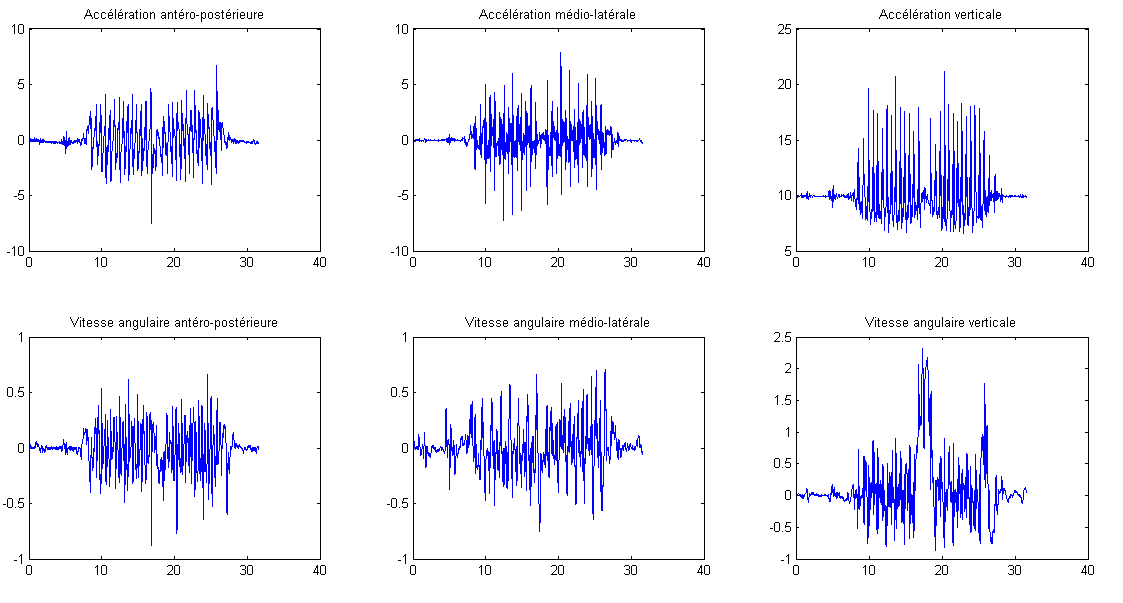
\includegraphics[scale=0.5]{ex_signal_back.png}
		\caption{Un exemple de signal de marche (enregistré à la ceinture)}
		\label{ex_signal_back}
	\end{figure}
	
	Sur ces signaux apparaissent de manière claire les différentes phases de l'expérience :
	\begin{itemize}
		\item Dans un premier temps, le patient est à l'arrêt, les 6 signaux sont quasiment constants (on n'observe que du bruit)
		\item Dans une seconde phase, le patient commence à marcher : on observe une phase transitoire entre l'arrêt et la marche dite de croisière
		\item La troisième phase de l'expérience correspond à la marche de croisière : le patient effectue une dizaine de mètres
		\item On observe ensuite le demi-tour (particulièrement sur les composantes verticales du signal), qui dure environ 1 seconde
		\item Puis, on a une nouvelle phase de marche, retour cette fois-ci
		\item Finalement, le patient s'arrête : on a à nouveau une phase transitoire, puis l'arrêt total du patient (où il ne reste plus que du bruit)
	\end{itemize}
	
	\vspace{1pc}
	
	Partant de ces constatations, on peut donc constater que les signaux acquis par les centrales inertielles peuvent être segmentés, qu'on peut isoler les différentes phases de l'expérience. Sur un signal, cela peut être fait de manière manuelle ; néanmoins, pour un neurologue enregistrant de manière régulière ce type d'expérience, il est concevable de désirer des algorithmes robustes permettant de traiter de manière automatique le problème de la détection des points de changement, décomposant ainsi le signal en sous-signaux correspondant à chacune des phases de l'expérience, afin de pouvoir les analyser séparément.
	
	\section{Formalisme mathématique}
	Afin de pouvoir traiter mathématiquement le problème, il nous faut tout d'abord poser des définitions claires sur l'objet du problème : il s'agit donc de définir ce qu'est une rupture, au sens mathématique.
	\\ \\
	La littérature propose une approche statistique du problème : on considère les signaux comme la réalisation d'une suite (finie) de variables aléatoires :
%Proposer ici des références bibliographiques...
	\begin{equation}
		(x_i)_{i \in \{1..N\}} = (X_i(\omega))_{i \in \{1..N\}}
		\label{11}
	\end{equation}
	
	Ce formalisme, qui peut paraître quelque peu abstrait en première approche, permet d'exprimer de manière simple la notion de rupture dans un signal.
	\\ \\
	Sur les signaux précédents, on constate, par exemple, une différence nette d'écart-type entre la phase à l'arrêt et la phase de marche ; de même, sur la vitesse angulaire verticale, on constate un changement de moyenne entre les phases de marche et le demi-tour. Il paraît donc naturel de considérer la distribution statistique des différents points d'un signal multivarié pour formaliser le concept de rupture.
	\\ \\
	On comprend alors la définition donnée par la littérature d'un point de rupture à un instant $t_0$ :
	\begin{equation}
	\begin{array}{ll}
			\forall t \in [1, t_0-1], X_i \sim p_1 \\
			 \forall t \in [t_0, N], X_i \sim p_2 \\
	\end{array}
	\end{equation}
	%Ref. needed
	
	On généralise de manière évidente au cas de $n$ ruptures aux points $(t_i)_{i \in \{0, n-1\}}$ :
	
	\begin{equation}
	\begin{array}{lll}
		\forall i \in \{0, n-1\}, \\
		\forall t \in \{t_{i-1}, t_i-1\}, X_i \sim p_i \\
		\forall t \in \{t_i, t_{i+1}-1\}, X_i \sim p_{i+1}
	\end{array}
	\label{multi_rupt}
	\end{equation}
	Où l'on a posé : $t_{-1} = 1$ et $t_n = N$.
	\\ \\
	Ce problème étant formalisé, il s'agit maintenant de trouver des méthodes pour détecter ces points de rupture.
	
	\chapter{Algorithme CUSUM : résolution du cas d'une seule rupture}
	
	
	\section{Principe de l'algorithme CUSUM}
	L'algorithme CUSUM fut proposé en 1954 par E.S. Page dans l'article \textit{Continuous Inspection Scheme}, dans une version en ligne. Les signaux étant ici déjà réalisés, il nous faut ici adapter l'algorithme au cas hors ligne (cf. M. Basseville, I.V. Nikiforov, \textit{Detection of Abrupt Changes : Theory and Application}).
	% \textit à remplacer par des \ref
	\\ \\
	Dans le formalisme précédent, on conçoit que les méthodes de détection de rupture se fondent sur des outils statistiques. L'idée de base de l'algorithme CUSUM hors ligne est la suivante : comparer l'hypothèse qu'il existe une rupture dans le signal considéré à l'hypothèse qu'il n'y en a pas. L'outil utilisé pour cette comparaison est la notion de vraisemblance. Pour simplifier, on fera maintenant l'hypothèse d'indépendance des variables aléatoires $(X_i)_{i \in [1,N]}$.
	\\ \\
	La fonction de vraisemblance quantifie la vraisemblance d'une hypothèse étant donnée une observation. Ici, l'observation faite est le signal, qui est la réalisation d'un nombre fini de variables aléatoires. On cherche à comparer l'hypothèse $H_t$ qu'à l'instant $t \in [1, N]$, il y a une rupture, à l'hypothèse $H_0$ qu'il n'y en a pas dans le signal. Les vraisemblances de ces hypothèses sont :
	\begin{equation}
	\begin{array}{ll}
		\forall t \in [1, N],l(H_t) = \prod_{i = 1}^{t-1} p_1(x_i) \prod_{i = t}^{N} p_2(x_i) \\
		l(H_0) = \prod_{i = 1}^N \tilde{p_0}(x_i) \\
	\end{array}	
	\end{equation}
	
	Introduisons alors le rapport de vraisemblance des hypothèses :
	\begin{equation}
		\forall t \in [1, N], \Lambda_t = \frac{l(H_t)}{l(H_0)} = \frac{\prod_{i = 1}^{t-1} p_1(x_i) \prod_{i = t}^{N} p_2(x_i)}{\prod_{i = 1]}^{N} \tilde{p_0}(x_i)}
	\end{equation}
	
	Pour simplifier, on fera ici l'hypothèse que nos lois sont issues d'une famille de lois indexée par un paramètre $\theta \in \mathbb{R}^d$. On a ainsi :
	
	\begin{equation*}
		p_1 = p_{\theta_1} ; p_2 = p_{\theta_2}
	\end{equation*}
	
	On ne connaît pas, a priori, les paramètres $\theta_1$ et $\theta_2$. Pour les estimer, on va donc utiliser l'estimation du maximum de vraisemblance. Il en découle alors la formule suivante, à la base de l'algorithme CUSUM, qui donne le logarithme du rapport de vraisemblance (\textit{log-likelihood ratio}, en anglais) :
	
	\begin{equation}
		\forall t \in [1, N], L_t=\ln\left[\frac{\left(\sup_{\theta_1}\prod_{i=1}^{t-1}p_{\theta_1}(y_i)\right)\left(\sup_{\theta_2}\prod_{i=t}^Np_{\theta_2}(y_i)\right)}{\sup_{\theta_0}p_{\theta_0}(y_i)}\right]
		\label{log_likelihood_ratio}
	\end{equation}
	
	Finalement, l'instant où il est le plus probable de trouver une rupture est celui qui maximise $L_t$. Ainsi, l'estimation par CUSUM du point de rupture d'un signal est :
	
	\begin{equation}
		\hat{t_0}=\arg\max_{1\le t\le N}L_t
	\end{equation}
	
	\section{Simplification dans le cas de distributions gaussiennes}
	Dans le cas général, la formule \ref{log_likelihood_ratio} est peu exploitable en raison de la présence de bornes supérieures. Afin de simplifier le problème des estimateurs au maximum de vraisemblance, on peut se proposer de faire une hypothèse sur la famille de lois $(p_\theta)_{\theta \in \mathbb{R}^d}$.
	\\ \\
	On suppose donc, à partir de maintenant, que chacune des variables aléatoires qui composent le signal suit une loi gaussienne, soit :
	
	\begin{equation*}
		p_{\mu, \sigma}(y) = \frac1{\sqrt{2 \pi} \sigma} \exp \left[ -\frac12 \left( \frac{y - \mu}{\sigma} \right)^2 \right]
	\end{equation*}
	
	Les estimateurs aux maximas de vraisemblance de la loi normale sont alors connus (cf. Larry Wasserman, \textit{All of Statistics : A concise course in statistical inference} par exemple) :
	\begin{equation}
	\left\{
	\begin{array}{ll}
		\hat{\mu} = \frac{1}{n} \sum_{i=1}^n x_i \\
		\hat{\sigma} = \sqrt{\frac{1}{n} \sum_{i=1}^n (x_i - \hat{\mu})^2} \\
	\end{array}
	\right.
	\label{estimators}
	\end{equation}
	
	Ceci nous permet alors de simplifier l'expression de $L_t$. Notons que l'hypothèse du gaussien ramène le problème du changement de loi à trois cas : changement de moyenne, changement d'écart-type, et changement de moyenne et d'écart-type.
	
	\subsection{Changement en moyenne}
	Faisant l'hypothèse d'un écart-type constant sur l'ensemble du signal, le paramètre $\theta$ est ici uniquement la moyenne $\mu$. \ref{log_likelihood_ratio} se réécrit donc, pour $t \in [1,N]$ :
	
	\begin{equation*}
	\begin{array}{ll}
		L_t = \sum_{i=1}^{t-1} \left[-\ln (\sqrt{2 \pi} \sigma)-\frac{1}{2}\left( \frac{y_i-\hat{\mu_1}}{\sigma} \right) ^2 \right] + \sum_{i=t}^{N} \left[-\ln (\sqrt{2 \pi} \sigma)-\frac{1}{2}\left( \frac{y_i-\hat{\mu_2}}{\sigma} \right) ^2 \right] \\
		~~~~~~~~~~~~~~~~~~~~~~~~ - \sum_{i=1}^{N} \left[-\ln (\sqrt{2 \pi} \sigma)-\frac{1}{2}\left( \frac{y_i-\hat{\mu_0}}{\sigma} \right) ^2 \right] \\
	\end{array}
	\end{equation*}
	
	Après calculs (À PRÉCISER ICI), on obtient :
	\begin{equation}
		\forall t \in [1, N], L_t = \frac{1}{2 \sigma ^2}\left[(t-1)\hat{\mu_1}^2 + (N - t + 1)\hat{\mu_2}^2 - N\hat{\mu_0}^2 \right]
		\label{meanchange}
	\end{equation}
	
	\subsection{Changement en écart-type}
	Faisant cette fois l'hypothèse d'une moyenne constante sur l'ensemble du signal, le paramètre $\theta$ est ici uniquement l'écart-type $\sigma$. \ref{log_likelihood_ratio} se réécrit donc, pour $t \in [1, N]$ :
	
	\begin{equation*}
	\begin{array}{ll}
			L_t = \sum_{i=1}^{t-1} \left[-\ln (\sqrt{2 \pi} \hat{\sigma_1}-\frac{1}{2}\left( \frac{y_i-\mu}{\hat{\sigma_1}} \right) ^2 \right] + \sum_{i=t}^{N} \left[-\ln (\sqrt{2 \pi} \hat{\sigma_2)}-\frac{1}{2}\left( \frac{y_i-\mu}{\hat{\sigma_2}} \right) ^2 \right] \\
			~~~~~~~~~~~~~~~~~~~~~~~~ - \sum_{i=1}^{N} \left[-\ln (\sqrt{2 \pi} \hat{\sigma_0})-\frac{1}{2}\left( \frac{y_i-\mu}{\hat{\sigma_0}} \right) ^2 \right] \\
		\end{array}
	\end{equation*}
	
	Ainsi :
	\begin{equation*}
	L_t=
	-\frac 12\left[\frac 1{\hat{\sigma_1}^2}\sum_{i=1}^{t-1}(y_i-\mu)^2
	+\frac 1{\hat{\sigma_2}^2}\sum_{i=t}^N(y_i-\mu)^2
	-\frac 1{\hat{\sigma_0}^2}\sum_{i=1}^N(y_i-\mu)^2\right]\]
	\[~~~~~~~~~~~~~~~~~~~~~~~~+N\ln(\hat{\sigma_0})-(k-1)\ln(\hat{\sigma_1})-(N-k+1)\ln(\hat{\sigma_2})
	\end{equation*}
	
	En vertu de \ref{estimators}, le premier terme de la somme se simplifie : il est en effet nul. On obtient alors : 
	
	\begin{equation}
		\forall t \in [1, N], L_t = N\ln (\hat{\sigma_0}) - (t-1)\ln (\hat{\sigma_1}) - (N-t+1)\ln (\hat{\sigma_2})
		\label{stdchange}
	\end{equation}
	
	\subsection{Changement en moyenne et en écart-type}
	Dans ce dernier cas, on doit estimer à la fois la moyenne et l'écart-type des différentes portions du signal. Les calculs sont identiques à ceux menés dans le cas d'un changement en écart-type, à la différence près que l'on a trois estimateurs différents sur la moyenne. On obtient un résultat quasiment identique :
	\begin{equation}
		\forall t \in [1,N], L_t = N\ln (\hat{\sigma_0}) - (t-1) \ln (\hat{\sigma_1}) - (N - t + 1) \ln (\hat{\sigma_2})
		\label{bothchange}
	\end{equation}
	La seule différence intervient dans l'estimateur de l'écart-type : au lieu d'utiliser un estimateur de moyenne sur l'ensemble du signal (ce qui est légitime si l'on fait l'hypothèse d'une moyenne constante), on utilise ici des estimateurs différents pour la moyenne sur chaque portion du signal.
	
	\section{Mise en œuvre sur des cas particuliers}
	Nous n'allons pas immédiatement traîter les signaux physiologiques vus précédemment : ceux-ci comportent plusieurs ruptures, l'algorithme CUSUM ne permettant d'en détecter qu'une seule. Les signaux utilisés dans cette partie sont des signaux synthétiques, obtenus grâce à MATLAB.

	\subsection{Détection d'un changement d'écart-type}
	
	On se place dans le cas d'un changement en écart-type de $\sigma_1 = 1$ à $\sigma_2 = 3$, à l'instant $t_0 = 201$.
	
	\begin{figure}[h]
		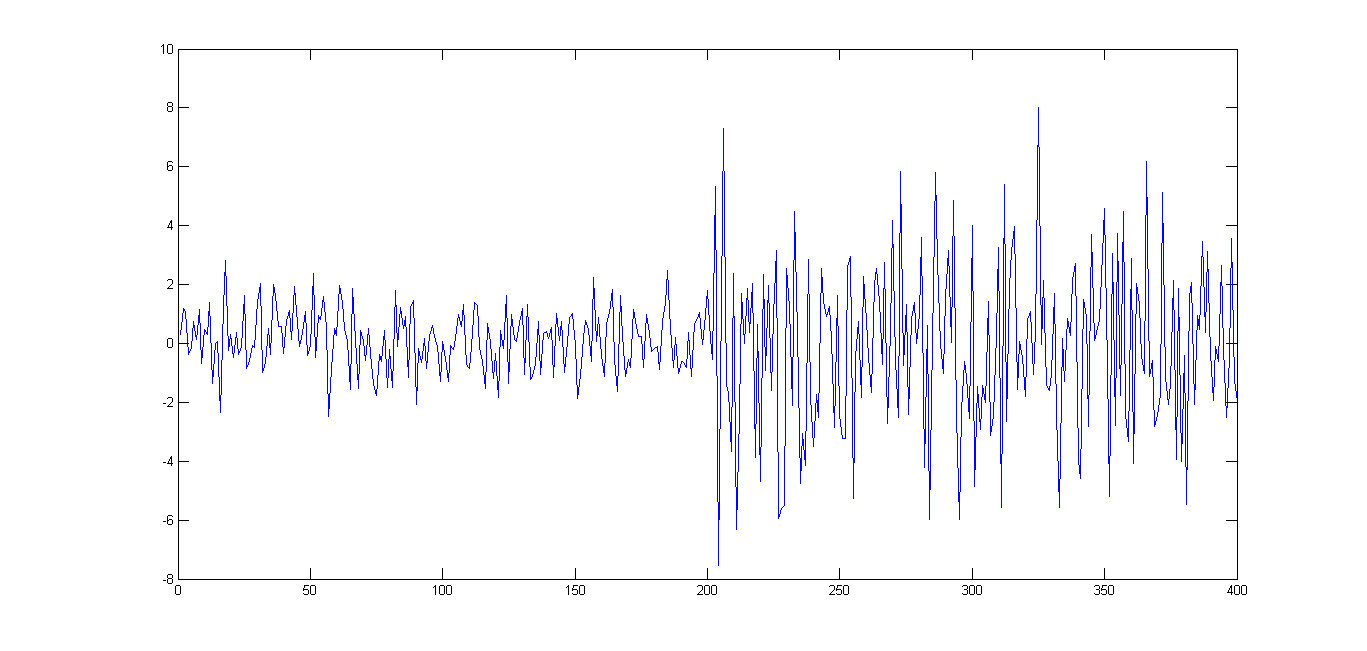
\includegraphics[scale=0.4]{test_signal_std.png}
		\caption{Pour $t \leq 200$, $X_t \sim \mathcal{N}(0, 1)$ ; pour $t > 200$, $X_t \sim \mathcal{N}(0, 3)$}
		\label{test_signal_std}
	\end{figure}
	
	L'équation \ref{stdchange} permet alors d'obtenir la figure \ref{llr_test_std}
	
	\begin{figure}[h]
		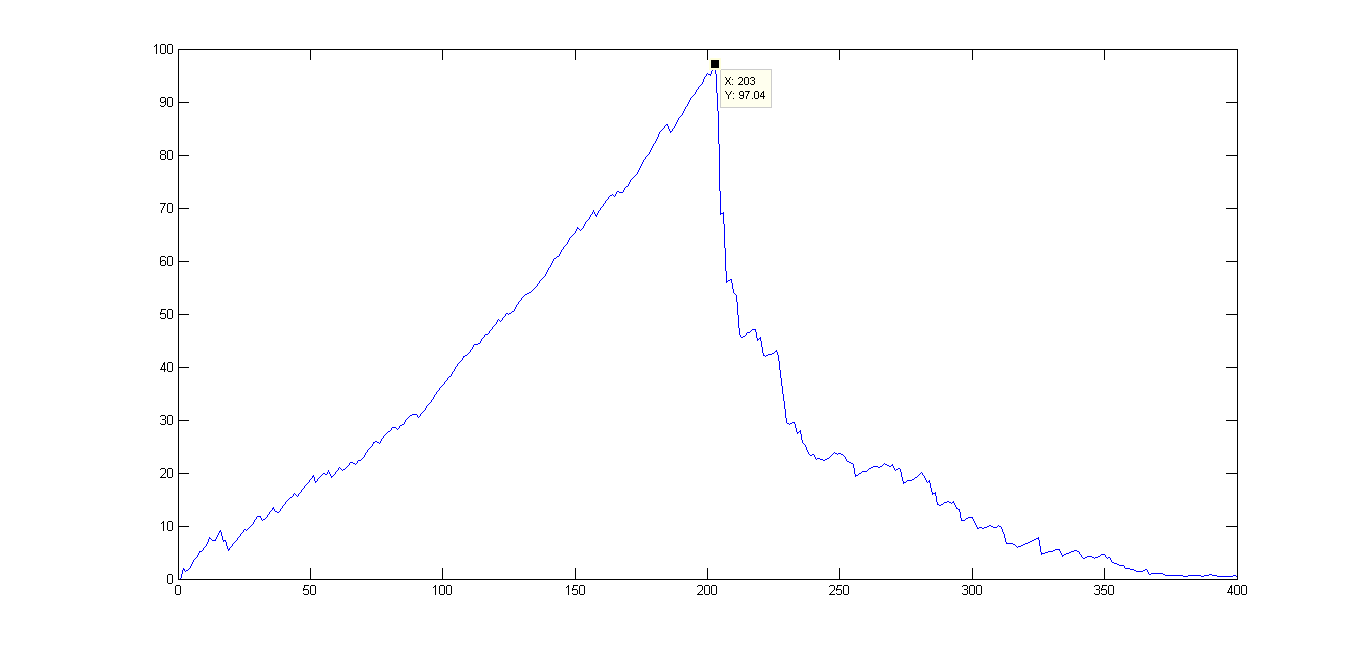
\includegraphics[scale=0.4]{llr_test_std.png}
		\caption{\textit{Log-likelihood ratio} du signal précédent}
		\label{llr_test_std}
	\end{figure}
	
	Ce comportement est le comportement typique de la courbe d'un \textit{log-likelihood ratio} sur un signal gaussien comportant une rupture. On observe ici que le maximum de la courbe est à l'instant 203, avec un \textit{log-likelihood ratio} $L_203 = 97,04$. On a donc l'estimateur par CUSUM du point de rupture :
	\begin{equation*}
		\hat{t_0} = 203 ; \hat{t_0} - t_0 = 2;
	\end{equation*}
	
	Ainsi, l'estimateur de points de rupture par CUSUM semble robuste dans le cas d'un changement par écart-type. Pour quantifier cette robustesse, on peut s'appuyer sur la déviation quadratique moyenne de cet estimateur (RMSD) : pour 5.000 signaux différents suivant les caractéristiques précédentes, on trouve $RMSD = 2,605$.
	
	\subsection{Détection d'un changement de moyenne}
	On se place dans le cas d'un changement en moyenne de $\mu_1 = 10$ à $\mu_2 = 20$, avec $t_0 = 201$.
	
	\begin{figure}[h]
		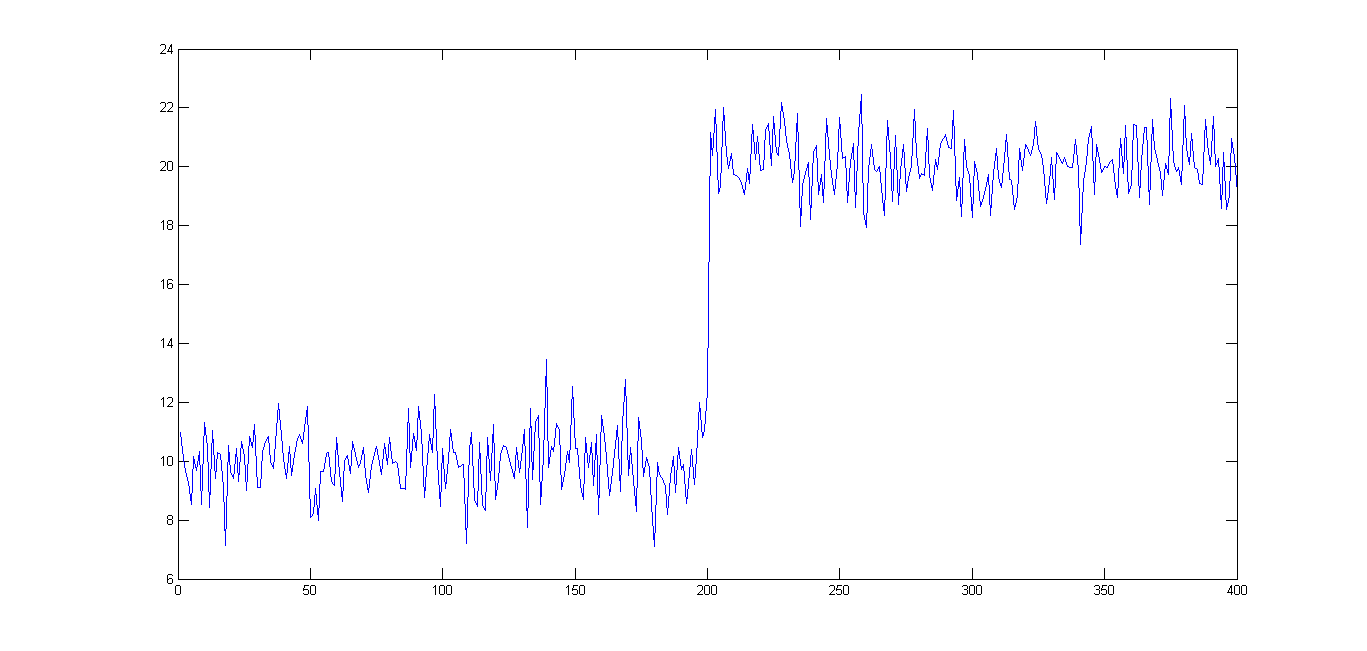
\includegraphics[scale=0.4]{test_signal_mean.png}
		\caption{Pour $t \leq 200$, $X_t \sim \mathcal{N}(10, 1)$ ; pour $t > 200$, $X_t \sim \mathcal{N}(20, 1)$}
		\label{test_signal_mean}
	\end{figure}
	
	On utilise cette fois l'équation \ref{meanchange} pour obtenir la figure \ref{llr_test_mean}.
	
	\begin{figure}[h]
		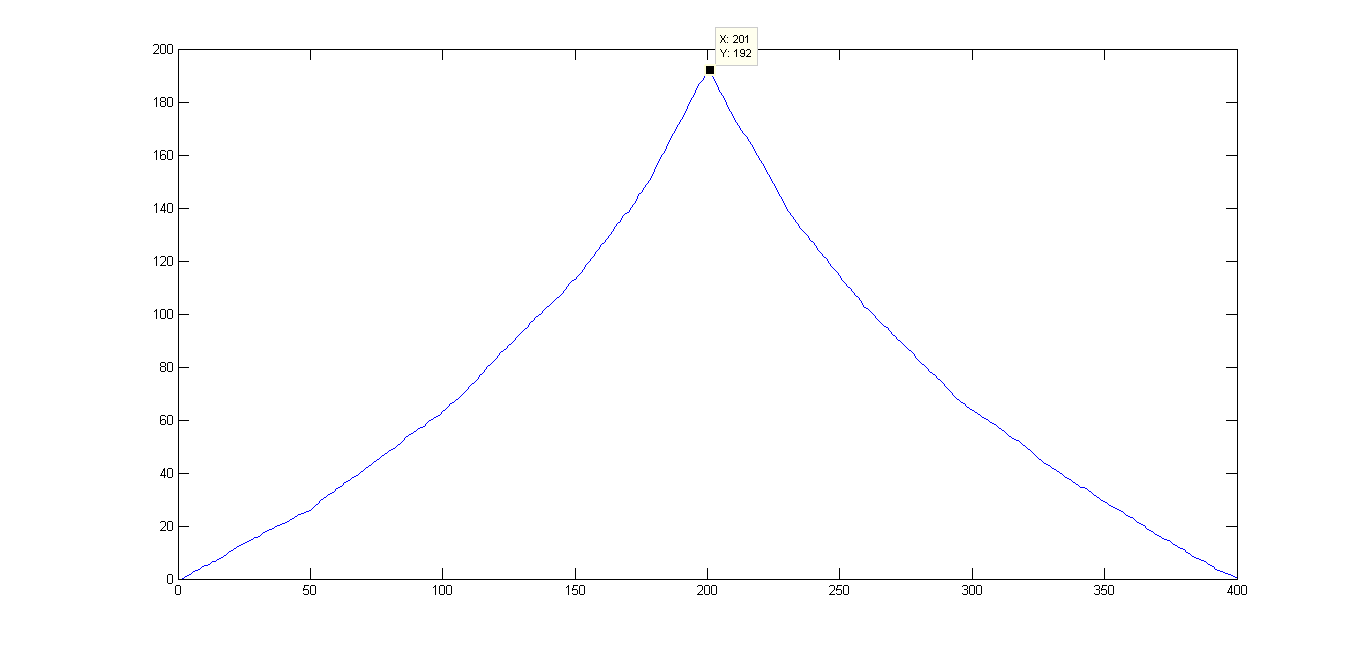
\includegraphics[scale=0.4]{llr_test_mean.png}
		\caption{\textit{Log-likelihood ratio} du signal précédent}
		\label{llr_test_mean}
	\end{figure}
	
	On obtient donc ici l'estimateur du point de rupture par CUSUM, avec un score de 192 :
	\begin{equation*}
		\hat{t_0} = 201 ; \hat{t_0} - t_0 = 0
	\end{equation*}
	
	De même que dans le cas précédent, on observe la robustesse de l'estimateur par CUSUM du point de rupture de ce signal. De la même manière que précédemment, en répétant 5.000 fois l'expérience précédente, on trouve : $RMSD = 0$.
	
	\chapter{Cas de plusieurs ruptures : implémentation dichotomique}
	Nous avons déjà présenté, dans le premier chapitre, le formalisme statistique associé au cas de plusieurs ruptures dans un signa (cf. équation \ref{multi_rupt}).
	
	
	\chapter{Cas de plusieurs ruptures : implémentation par fenêtres}
	
	\chapter{Évaluation des performances}
	
	\chapter{Conclusion}
\end{document}
